%
% Presentación de TT uno.
% Proyecto Lovelace.
% Planteamiento de la solución.
%

\section{Planteamiento de la solución}

\subsection{Objetivos del proyecto} % =========================================
\begin{frame}{Objetivos del proyecto}

  Lo que se busca con este proyecto es implementar un programa generador de
  \textit{tokens} que provea confidencialidad a los datos de las tarjetas
  bancarias.

  Además, con el afán de disminuir la desinformación existente sobre la
  tokenización, se busca obtener una comparativos de los algoritmos
  implementados.
  
\end{frame}

\subsection{Metodología del proyecto} % =======================================
\begin{frame}{Metodología del proyecto}

  Para el desarrollo de este proyecto se está usando una metodología de
  prototipos, en la que cada prototipo usa como metodología interna SDL
  (\textit{Security Development Lifecycle}).

  SDL es una metodología especializada para software de seguridad desarrollada
  por Microsoft, que se caracteriza por continuas fases de verificación de
  seguridad y una primera etapa de estudio de los temas acordes al proyecto.
  
\end{frame}

\subsection{Prototipos} % =====================================================
\begin{frame}{Prototipos}
  
  Este proyecto está dividido en 3 prototipos, los cuales son:

  \begin{figure}[H]
    \begin{center}
      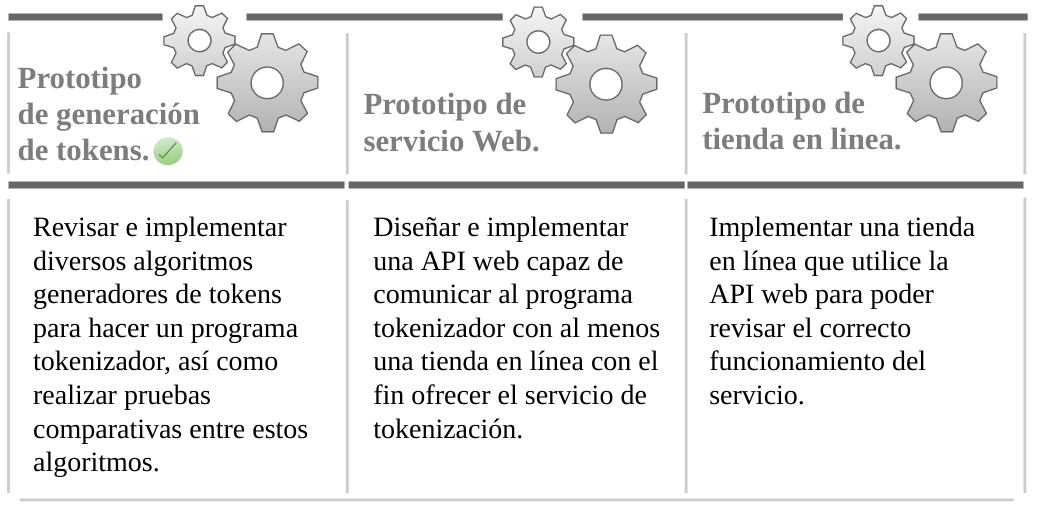
\includegraphics[width=1.0\linewidth]{diagramas/prototipos.png}
      \caption{Prototipos del trabaja terminal.}
    \end{center}
  \end{figure}

\end{frame}

\subsection{Prototipo de generación de tokens} % ==============================
\begin{frame}{Prototipo de generación de tokens}

  En TT1 se planeó terminar el primer prototipo dado que es la parte
  central del proyecto; situación que se consiguió, llegando a implementar
  5 algoritmos distintos y realizar pruebas comparativas entre estos.
  Además, en los algoritmos pertinentes, se realizaron pruebas de
  aleatoriedad con el fin de respaldar la seguridad de la implementación.

\end{frame}

\subsection{Especificaciones técnicas del desarrollo} % ========================
\begin{frame}{Especificaciones técnicas del desarrollo}

  La implementación de los algoritmos generadores de \textit{tokens} se hizo
  en lenguaje C++, dado que combina mantenibilidad y el nivel de rendimiento
  que ofrece.

  Para las implementación que hicieran uso de una base de datos, se utilizó
  el gestor MariaDB, el cual es una bifurcación de MySQL. 

\end{frame}
